% Options for packages loaded elsewhere
\PassOptionsToPackage{unicode}{hyperref}
\PassOptionsToPackage{hyphens}{url}
%
\documentclass[
]{article}
\usepackage{amsmath,amssymb}
\usepackage{lmodern}
\usepackage{setspace}
\usepackage{iftex}
\ifPDFTeX
  \usepackage[T1]{fontenc}
  \usepackage[utf8]{inputenc}
  \usepackage{textcomp} % provide euro and other symbols
\else % if luatex or xetex
  \usepackage{unicode-math}
  \defaultfontfeatures{Scale=MatchLowercase}
  \defaultfontfeatures[\rmfamily]{Ligatures=TeX,Scale=1}
\fi
% Use upquote if available, for straight quotes in verbatim environments
\IfFileExists{upquote.sty}{\usepackage{upquote}}{}
\IfFileExists{microtype.sty}{% use microtype if available
  \usepackage[]{microtype}
  \UseMicrotypeSet[protrusion]{basicmath} % disable protrusion for tt fonts
}{}
\makeatletter
\@ifundefined{KOMAClassName}{% if non-KOMA class
  \IfFileExists{parskip.sty}{%
    \usepackage{parskip}
  }{% else
    \setlength{\parindent}{0pt}
    \setlength{\parskip}{6pt plus 2pt minus 1pt}}
}{% if KOMA class
  \KOMAoptions{parskip=half}}
\makeatother
\usepackage{xcolor}
\usepackage[left=2cm,right=2cm,top=2cm,bottom=2cm]{geometry}
\usepackage{longtable,booktabs,array}
\usepackage{calc} % for calculating minipage widths
% Correct order of tables after \paragraph or \subparagraph
\usepackage{etoolbox}
\makeatletter
\patchcmd\longtable{\par}{\if@noskipsec\mbox{}\fi\par}{}{}
\makeatother
% Allow footnotes in longtable head/foot
\IfFileExists{footnotehyper.sty}{\usepackage{footnotehyper}}{\usepackage{footnote}}
\makesavenoteenv{longtable}
\usepackage{graphicx}
\makeatletter
\def\maxwidth{\ifdim\Gin@nat@width>\linewidth\linewidth\else\Gin@nat@width\fi}
\def\maxheight{\ifdim\Gin@nat@height>\textheight\textheight\else\Gin@nat@height\fi}
\makeatother
% Scale images if necessary, so that they will not overflow the page
% margins by default, and it is still possible to overwrite the defaults
% using explicit options in \includegraphics[width, height, ...]{}
\setkeys{Gin}{width=\maxwidth,height=\maxheight,keepaspectratio}
% Set default figure placement to htbp
\makeatletter
\def\fps@figure{htbp}
\makeatother
\setlength{\emergencystretch}{3em} % prevent overfull lines
\providecommand{\tightlist}{%
  \setlength{\itemsep}{0pt}\setlength{\parskip}{0pt}}
\setcounter{secnumdepth}{5}
\usepackage{lineno}
\linenumbers
\newcommand{\beginsupplement}{\setcounter{table}{0}  \renewcommand{\thetable}{S\arabic{table}} \setcounter{figure}{0} \renewcommand{\thefigure}{S\arabic{figure}}}
\usepackage{float}
\ifLuaTeX
  \usepackage{selnolig}  % disable illegal ligatures
\fi
\IfFileExists{bookmark.sty}{\usepackage{bookmark}}{\usepackage{hyperref}}
\IfFileExists{xurl.sty}{\usepackage{xurl}}{} % add URL line breaks if available
\urlstyle{same} % disable monospaced font for URLs
\hypersetup{
  pdftitle={IMF and Benchmark Forecasts},
  hidelinks,
  pdfcreator={LaTeX via pandoc}}

\title{IMF and Benchmark Forecasts}
\author{}
\date{\vspace{-2.5em}}

\begin{document}
\maketitle

\setstretch{2}
\hypertarget{this-document}{%
\section{This document}\label{this-document}}

Here we document the proportion of true values that ``miss'' the 50\% and 80\% central prediction intervals - that is, the proportions of observations that falls \textit{below} the 0.1-quantile and 0.25-quantile and the proportion that falls \textit{above} the 0.75-quantile and 0.9-quantile.

The respective proportions are calculated separately for each forecast source (IMF, ar, bvar, bvarqu\footnote{bvarqu denotes the quantile forecasts that are taken directly from the BVAR model, while bvar denotes the quantile forecasts that are drawn from past point forecast errors of the BVAR model (analagously to the IMF and ar forecasts)}, target (GDP Growth and Inflation) and horizon (0 - ``Fall, same year'' to 1.5 - ``Spring, previous year''). We treat absolute error handling as the default, and show results for directional error handling in the same respective source's color, but in a lighter shade. This plot is shown on page 3, with desired nominal exceedance proportions shown as dashed lines.

On page 4, we also plot exceedance levels for the bvarqu model separately for two equally sized parts of the time period under study. Differences in coverage between the two time periods at the respective quantile levels seem non-substantial.

\hypertarget{gdp-growth-forecasts}{%
\section{GDP growth forecasts}\label{gdp-growth-forecasts}}

Overall, the forecasts that stem (a) from the directional error methods for the ar and bvar forecasts and (b) the IMF forecasts in general tend to be better calibrated, especially at the lower quantile levels.

The bvarqu forecasts show relatively large\footnote{in relation to the respective desired nominal level} exceedance proportions at the lower quantile levels (q = 0.1, q = 0.25) and small exceedance proportions at the upper quantile levels, an indication of overprediction. The respective forecast intervals ``cover too much ground'' in the direction of positive deviations of the realized values from the point prediction, while simultaneously ``covering too little'' in the other direction. Similarly, this is also an issue for the absolute ar, bvar and (albeit to a slightly lesser extent) IMF forecasts.

Lastly, the bvarqu forecasts appear to be too narrow at the shortest horizon (0 - ``Fall, same year'') only, since they show relatively large exceedances at both the lower and the upper quantile levels.

\hypertarget{inflation-forecasts}{%
\section{Inflation forecasts}\label{inflation-forecasts}}

For the inflation forecasts, the bvarqu model (along with absolute ar and bvar to a lesser extent) show small exceedance proportions at the upper quantiles, especially for the 0.9-quantile and larger horizons, indicating intervals that are too long in the region above the point forecast. This also explains the aggregate near-zero underprediction scores for these methods (see other pdf).

Interestingly, the directional methods show the opposite issue, in that they have a too large proportion of exceedances at the upper quantile levels.

At the lower quantile levels, all methods appear to be better calibrated.

\hypertarget{overall}{%
\section{Overall}\label{overall}}

In summary, it appears that for GDP, the entire distributions seem to be biased (shifted) upwards for the bvarqu and absolute ar and bvar models. For inflation, it seems that they are just too long at the top, while being better calibrated at the bottom.

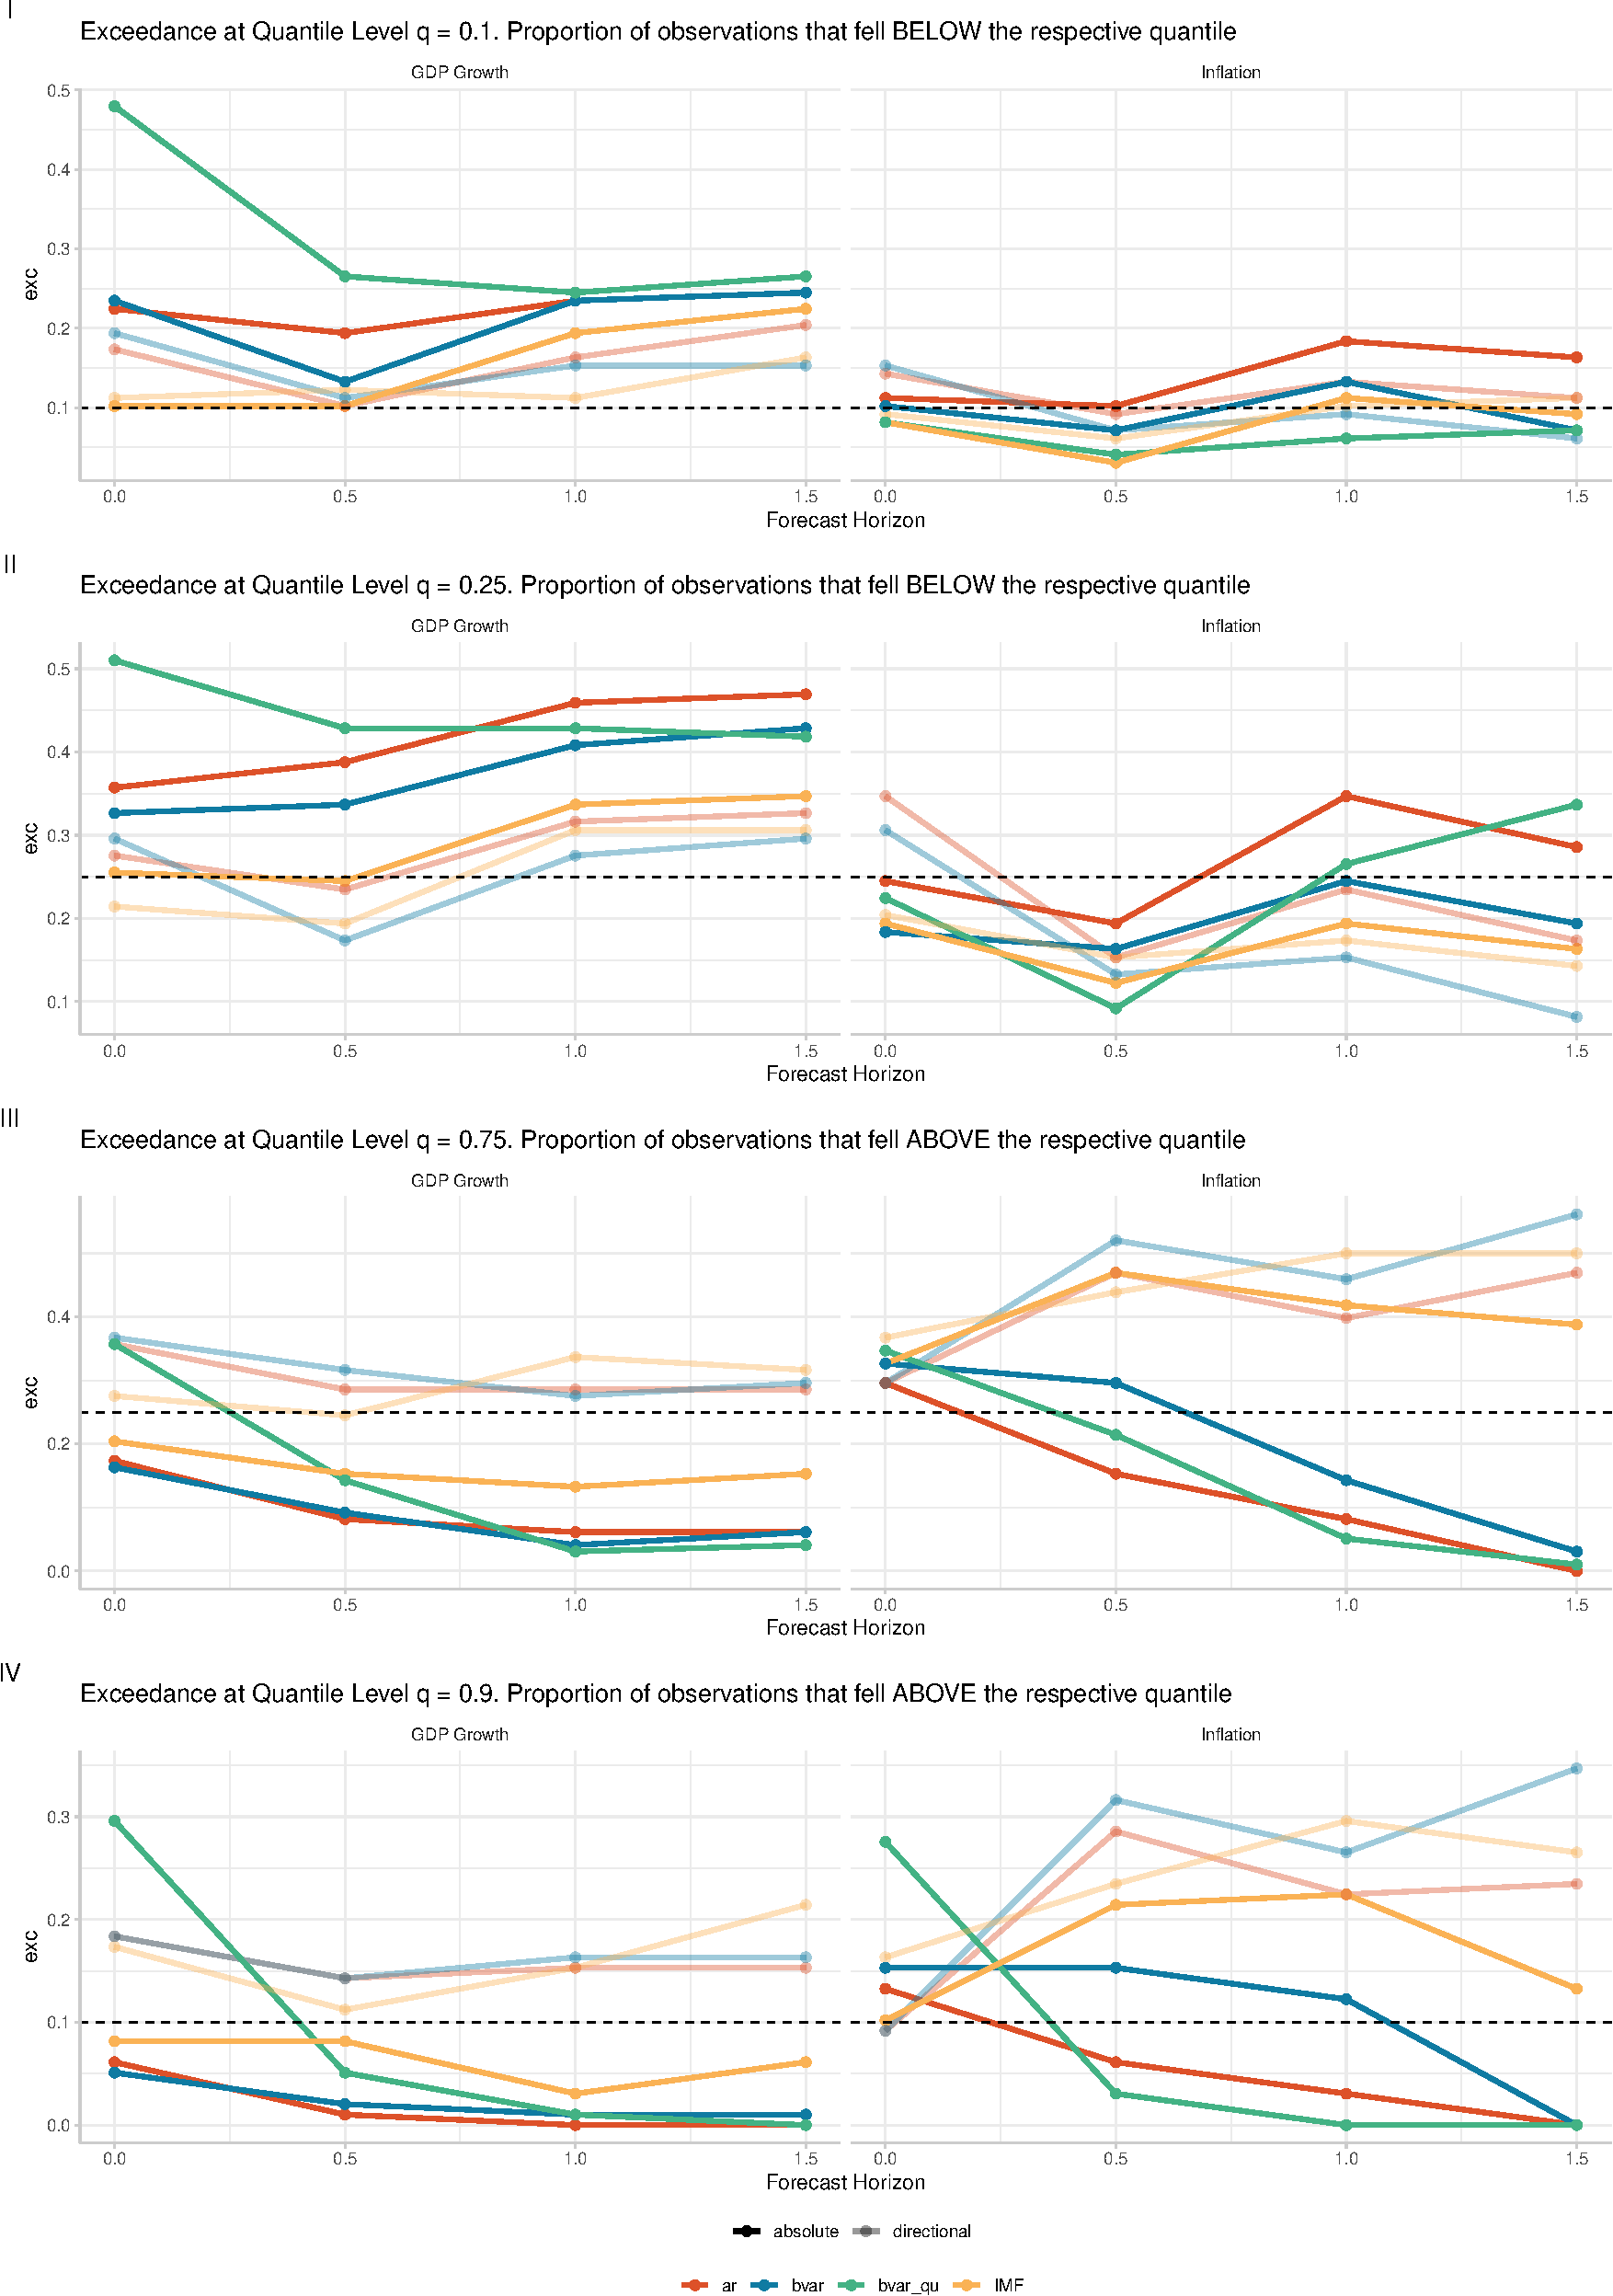
\includegraphics{quantile_coverage_files/figure-latex/unnamed-chunk-4-1.pdf}

\hypertarget{exceedance-for-bvarqu-by-time-period}{%
\section{Exceedance for bvarqu, by time period}\label{exceedance-for-bvarqu-by-time-period}}

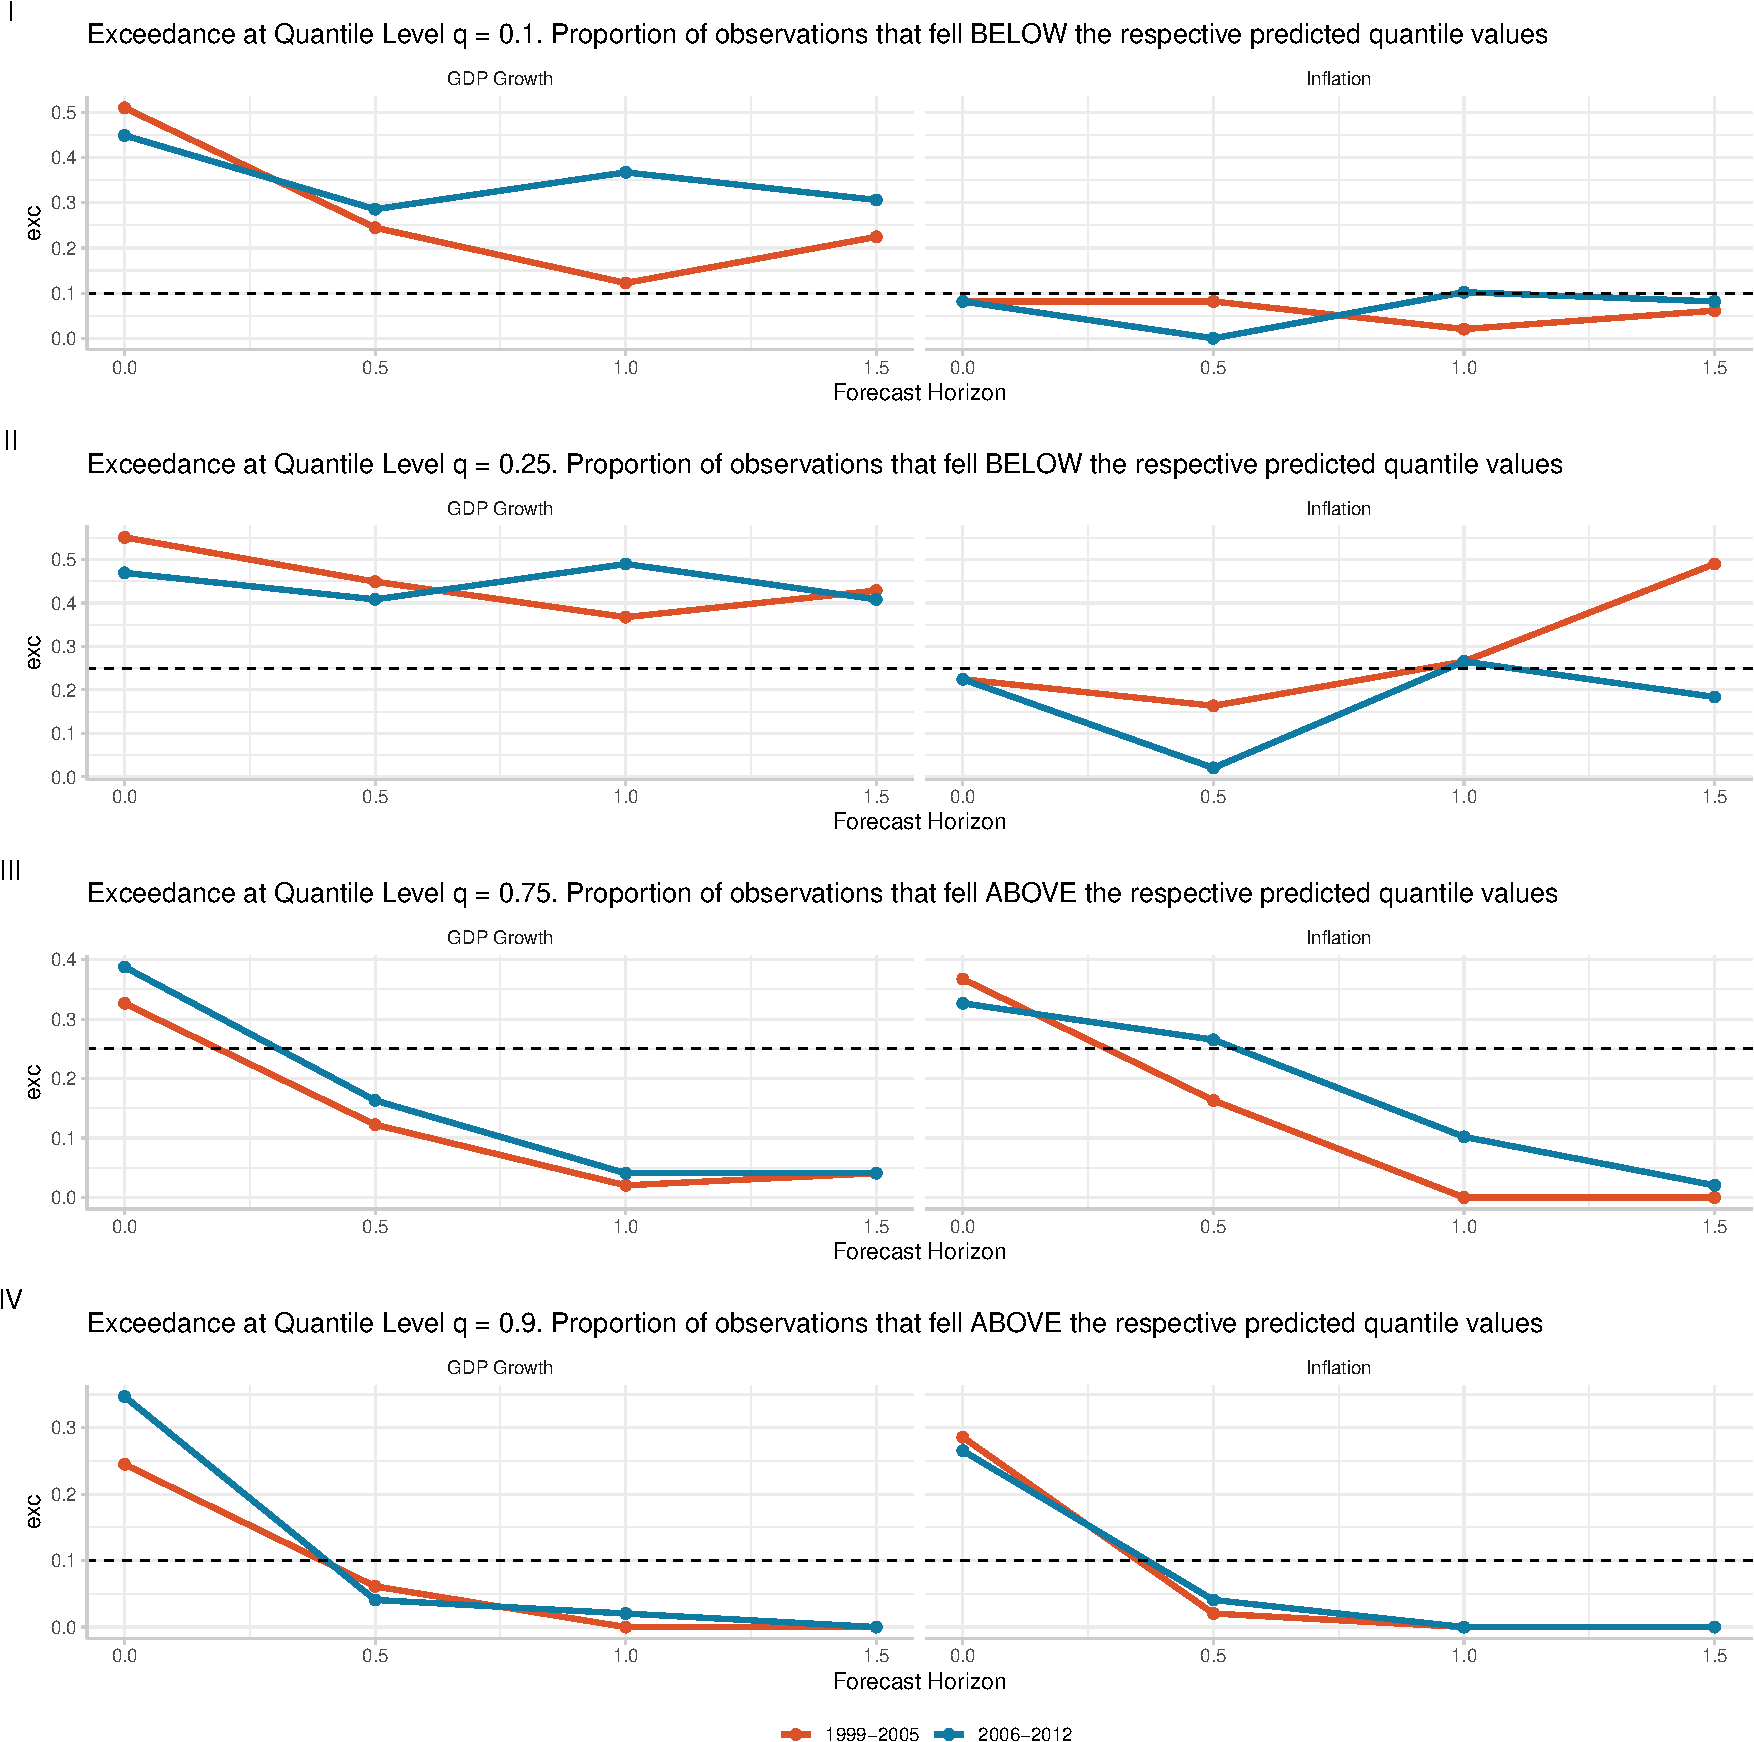
\includegraphics{quantile_coverage_files/figure-latex/unnamed-chunk-5-1.pdf}

\end{document}
